
\documentclass{article}

\usepackage{fancyhdr}
\usepackage{extramarks}
\usepackage{amsmath}
\usepackage{amsthm}
\usepackage{amsfonts}
\usepackage{tikz}
\usepackage[plain]{algorithm}
\usepackage{algpseudocode}
\usepackage{listings}
\usepackage{xcolor}
\usepackage[english]{babel}
\usepackage[T1]{fontenc}
\usepackage{lmodern,mathrsfs}
\usepackage{xparse}
\usepackage[inline,shortlabels]{enumitem}
\setlist{topsep=2pt,itemsep=2pt,parsep=0pt,partopsep=0pt}
\usepackage[dvipsnames]{xcolor}
\usepackage[utf8]{inputenc}
\usepackage[a4paper,top=0.5in,bottom=0.2in,left=0.5in,right=0.5in,footskip=0.3in,includefoot]{geometry}
\usepackage[most]{tcolorbox}
\tcbuselibrary{minted} % tcolorbox minted library, required to use the "minted" tcb listing engine (this library is not loaded by the option [most])
\usepackage{minted} % Allows input of raw code, such as Python code
% \usepackage[colorlinks]{hyperref}



\usetikzlibrary{automata,positioning}

%
% Basic Document Settings
%

\tcbset{
    pythoncodebox/.style={
        enhanced jigsaw,breakable,
        colback=gray!10,colframe=gray!20!black,
        boxrule=1pt,top=2pt,bottom=2pt,left=2pt,right=2pt,
        sharp corners,before skip=10pt,after skip=10pt,
        attach boxed title to top left,
        boxed title style={empty,
            top=0pt,bottom=0pt,left=2pt,right=2pt,
            interior code={\fill[fill=tcbcolframe] (frame.south west)
                --([yshift=-4pt]frame.north west)
                to[out=90,in=180] ([xshift=4pt]frame.north west)
                --([xshift=-8pt]frame.north east)
                to[out=0,in=180] ([xshift=16pt]frame.south east)
                --cycle;
            }
        },
        title={#1}, % Argument of pythoncodebox specifies the title
        fonttitle=\sffamily\bfseries
    },
    pythoncodebox/.default={}, % Default is No title
    %%% Starred version has no frame %%%
    pythoncodebox*/.style={
        enhanced jigsaw,breakable,
        colback=gray!10,coltitle=gray!20!black,colbacktitle=tcbcolback,
        frame hidden,
        top=2pt,bottom=2pt,left=2pt,right=2pt,
        sharp corners,before skip=10pt,after skip=10pt,
        attach boxed title to top text left={yshift=-1mm},
        boxed title style={empty,
            top=0pt,bottom=0pt,left=2pt,right=2pt,
            interior code={\fill[fill=tcbcolback] (interior.south west)
                --([yshift=-4pt]interior.north west)
                to[out=90,in=180] ([xshift=4pt]interior.north west)
                --([xshift=-8pt]interior.north east)
                to[out=0,in=180] ([xshift=16pt]interior.south east)
                --cycle;
            }
        },
        title={#1}, % Argument of pythoncodebox specifies the title
        fonttitle=\sffamily\bfseries
    },
    pythoncodebox*/.default={}, % Default is No title
}

% Custom tcolorbox for Python code (not the code itself, just the box it appears in)
\newtcolorbox{pythonbox}[1][]{pythoncodebox=#1}
\newtcolorbox{pythonbox*}[1][]{pythoncodebox*=#1} % Starred version has no frame

% Custom minted environment for Python code, NOT using tcolorbox
\newminted{python}{autogobble,breaklines,mathescape}

% Custom tcblisting environment for Python code, using the "minted" tcb listing engine
% Adapted from https://tex.stackexchange.com/a/402096
\NewTCBListing{python}{ !O{} !D(){} !G{} }{
    listing engine=minted,
    listing only,
    pythoncodebox={#1}, % First argument specifies the title (if any)
    minted language=python,
    minted options/.expanded={
        autogobble,breaklines,mathescape,
        #2 % Second argument, delimited by (), denotes options for the minted environment
    },
    #3 % Third argument, delimited by {}, denotes options for the tcolorbox
}

\topmargin=-0.45in
\evensidemargin=0in
\oddsidemargin=0in
\textwidth=6.5in
\textheight=9.0in
\headsep=0.25in

\linespread{1.1}

\pagestyle{fancy}
\lhead{\hmwkAuthorName}
\chead{\hmwkClass\ (\hmwkClassInstructor): \hmwkTitle}
\rhead{\firstxmark}
\lfoot{\lastxmark}
\cfoot{\thepage}

\renewcommand\headrulewidth{0.4pt}
\renewcommand\footrulewidth{0.4pt}

\setlength\parindent{0pt}

%
% Create Problem Sections
%

\newcommand{\enterProblemHeader}[1]{
	\nobreak\extramarks{}{Problem \arabic{#1} continued on next page\ldots}\nobreak{}
	\nobreak\extramarks{Problem \arabic{#1} (continued)}{Problem \arabic{#1} continued on next page\ldots}\nobreak{}
}

\newcommand{\exitProblemHeader}[1]{
	\nobreak\extramarks{Problem \arabic{#1} (continued)}{Problem \arabic{#1} continued on next page\ldots}\nobreak{}
	\stepcounter{#1}
	\nobreak\extramarks{Problem \arabic{#1}}{}\nobreak{}
}

\setcounter{secnumdepth}{0}
\newcounter{partCounter}
\newcounter{homeworkProblemCounter}
\setcounter{homeworkProblemCounter}{1}
\nobreak\extramarks{Problem \arabic{homeworkProblemCounter}}{}\nobreak{}

%
% Homework Problem Environment
%
% This environment takes an optional argument. When given, it will adjust the
% problem counter. This is useful for when the problems given for your
% assignment aren't sequential. See the last 3 problems of this template for an
% example.
%
\newenvironment{homeworkProblem}[1][-1]{
	\ifnum#1>0
		\setcounter{homeworkProblemCounter}{#1}
	\fi
	\section{Problem \arabic{homeworkProblemCounter}}
	\setcounter{partCounter}{1}
	\enterProblemHeader{homeworkProblemCounter}
}{
	\exitProblemHeader{homeworkProblemCounter}
}

%
% Homework Details
%   - Title
%   - Due date
%   - Class
%   - Section/Time
%   - Instructor
%   - Author
%

\newcommand{\hmwkTitle}{Problem Set\ \#1}
\newcommand{\hmwkDueDate}{Jun 15, 2025}
\newcommand{\hmwkClass}{ECON 124}
\newcommand{\hmwkClassInstructor}{Dr. Deniz Baglan}
\newcommand{\hmwkAuthorName}{\textbf{Alejandro Ouslan}}

%
% Title Page
%

\title{
	\vspace{2in}
	\textmd{\textbf{\hmwkClass:\ \hmwkTitle}}\\
	\normalsize\vspace{0.1in}\small{Due\ on\ \hmwkDueDate}\\
	\vspace{0.1in}\large{\textit{\hmwkClassInstructor}}
	\vspace{3in}
}

\author{\hmwkAuthorName}
\date{}

\renewcommand{\part}[1]{\textbf{\large Part \Alph{partCounter}}\stepcounter{partCounter}\\}

%
% Various Helper Commands
%

% Useful for algorithms
\newcommand{\alg}[1]{\textsc{\bfseries \footnotesize #1}}

% For derivatives
\newcommand{\deriv}[1]{\frac{\mathrm{d}}{\mathrm{d}x} (#1)}

% For partial derivatives
\newcommand{\pderiv}[2]{\frac{\partial}{\partial #1} (#2)}

% Integral dx
\newcommand{\dx}{\mathrm{d}x}

% Alias for the Solution section header
\newcommand{\solution}{\textbf{\large Solution}}

% Probability commands: Expectation, Variance, Covariance, Bias
\newcommand{\E}{\mathrm{E}}
\newcommand{\Var}{\mathrm{Var}}
\newcommand{\Cov}{\mathrm{Cov}}
\newcommand{\Bias}{\mathrm{Bias}}

\begin{document}

\maketitle

\pagebreak

% Homework problem 1
\begin{homeworkProblem}
  Consider two least-square Regressions
  $$y = X_1 \beta_1 + \epsilon$$
  and 
  $$y = X_1 \beta_1 + X_2 \beta_2 \epsilon$$
  Let $R_1^2$ and $R_2^2$ be the R+squared from the two regressions, respectively. Show
  that $R_2^2 \ge R_1^2$
  \begin{proof}
    \[
    \begin{split}
      R_1^2 \le R_2^2 &\Rightarrow 1- \frac{SSR_1}{TSS} \le 1-\frac{SSR_2}{TSS} \\
                      &\Rightarrow SSR_2 \le SSR_1 \\
                      &\Rightarrow ||(I - P_{X_2})y||^2 \le ||(I - P_{X_1})y||^2 \\
    \end{split}
    \]
    Given that $col(X_1) \subset col(X_2)$ and $P_{X_1}$ is a projection of $y$ onto the 
    subspace $col(X_1)$ then:
    \[
    \begin{split}
                      &\Rightarrow ||(I - P_{X_2})y||^2 \le ||(I - P_{X_1})y||^2 \\
                      &\Rightarrow SSR_2 \le SSR_1 \\
                      &\Rightarrow 1- \frac{SSR_1}{TSS} \le 1-\frac{SSR_2}{TSS} \\
                      &\Rightarrow R_1^2 \le R_2^2 
    \end{split}
    \]
  Thus $R_1^2 \le R_2^2$
  \end{proof}
\end{homeworkProblem}

% Homework Problem 2 
\begin{homeworkProblem}
  Use the cps09mar data for this question. The data set and the description file is 
  attached under the assignment of Canvas. Estimate a log wage regression for the subsample 
  of white male Hispanics. In addition to education, experience, and its square, include a set of binary 
  variables for Northeast, South and West so that Midwest is the exuded group. For marital status, create 
  variables for married, widow or divorced, and separated, so that single (never married) is the excluded 
  group.


\begin{table}[h!]
\centering
\begin{tabular}{lr}
\textbf{Variable} & \textbf{Coefficient} \\
\hline
Intercept         & 1.0019 \\
Education         & 0.0885 \\
North Dummy       & 0.0574 \\
South Dummy       & -0.0729 \\
West Dummy        & 0.0231 \\
Married Dummy     & 0.1682 \\
Widowed Dummy     & 0.1853 \\
Separated Dummy   & 0.0523 \\
Experience (exp)  & 0.0337 \\
Experience$^2$ (exp\_2) & -0.0004 \\
\end{tabular}
\caption{Estimated coefficients from regression model}
\end{table}

\begin{pythonbox}[Python Code]
	\inputminted{python}{code/reg3.py}
\end{pythonbox}

\end{homeworkProblem}

% Homework Problem 3 
\begin{homeworkProblem}
  The data koop tobias subsample is extracted from koop and tobias (2004) study
  of the relationship between wages and education, ability, and family characterises. 
  Et $X_1$ equal a constant, education, experience, and ability. Let $X_2$ contain
  the mothers education, the fathers education, and the number of siblings. Let $y$ 
  e the log of the hourly wage. Show you regression output

  \begin{enumerate}
    \item Compute the least square regression coefficients in the regression of $y$ on $X_1$.
      Report the coefficients. 
      \begin{table}[h!]
\centering
\begin{tabular}{lr}
\textbf{Variable} & \textbf{Coefficient} \\
\hline
Intercept   & 1.6636 \\
Education   & 0.0145 \\
Experience  & 0.0710 \\
Ability     & 0.0266 \\
\end{tabular}
\caption{Estimated coefficients for the regression model}
\end{table}

    \item Compute the least square regression coefficients in the regression of $y$ on $X_1$ 
      and $X_2$. Report the coefficients.
      \begin{table}[h!]
\centering
\begin{tabular}{lr}
\textbf{Variable} & \textbf{Coefficient} \\
\hline
Mother's Education  & 0.1028 \\
Father's Education  & 0.0490 \\
Siblings            & 0.0847 \\
\end{tabular}
\caption{Regression coefficients without intercept}
\end{table}

    \item Regress each of the three variables in $X_2$ on all the variables in  $X_1$ and copete 
      the residuals form each regression. Arrange these new variables in the (15X3) matrix $X_2^\star$. 
      What are the sample means of these three variables?
\[
X_2^\star =
\begin{bmatrix}
-0.8891 & -1.2215 & -0.6868 \\
-0.1152 & -1.7148 & 0.0547 \\
-0.4563 & 0.0457 & -2.1323 \\
-0.6006 & -2.5489 & 1.5568 \\
-0.0837 & -0.6653 & -1.2062 \\
-0.1541 & 3.2126 & -0.0721 \\
-0.1044 & -1.1987 & -0.5662 \\
0.2152 & 2.2027 & 0.0112 \\
-0.5327 & -1.1005 & 0.2349 \\
0.4595 & -0.5267 & -0.2678 \\
2.6149 & 3.0896 & 1.0509 \\
2.1254 & 0.7824 & 1.2776 \\
0.4188 & 0.2255 & 0.8159 \\
-0.8591 & -0.0135 & -0.7581 \\
-2.0388 & -0.5686 & 0.6875
\end{bmatrix}
\]
    \item Compute the $R^2$ for the regression of $y$ on $X_1$ and $X_2$. Repeat the computation for the 
      case in which the constant term is omitted from $X_1$. What happens to $R^2$? 
\begin{table}[!ht]
\centering
\begin{tabular}{ll}
\textbf{Regression Setup} & \(\boldsymbol{R^2}\) \\
With intercept included  (first model) & 0.1834 \\
With intercept included  (alternative) & 0.1916 \\
Without intercept included (firs model) & -0.3537 \\
Without intercept included (alternative) & -0.0219 \\
\end{tabular}
\caption{Values of \( R^2 \) under different regression setups}
\end{table}

When the intercept is included, the \( R^2 \) values are positive and reflect the proportion of variance explained by the model. However, when the intercept is omitted, some \( R^2 \) values become negative, indicating that the regression model fits the data worse than a simple horizontal line at the mean of \( y \).



    \item Compute the adjusted $R^2$ for the full regression including the constant term. 

\[
\text{Adjusted } R^2 = 0.1530
\]
  \end{enumerate}
  \begin{pythonbox}[Python Code]
	\inputminted{python}{code/reg3.py}
\end{pythonbox}


\end{homeworkProblem}

% Homework Problem 4
Suppose that you have two independent unbiased estimators of the same parameter $\theta$, say 
$\hat{\theta}_1$ and $\hat{\theta}_2$, with different variances $v_1$ and $v_2$, What linear combination 
$\hat{\theta} = c_1\hat{\theta_1} + c_2\hat{\theta}_2$ is the minimum variance unbiased estimator of 
$\theta$?
\[
\hat{\theta} = c_1 \hat{\theta}_1 + c_2 \hat{\theta}_2
\]
\[
E[\hat{\theta}] = c_1 E[\hat{\theta}_1] + c_2 E[\hat{\theta}_2] = c_1 \theta + c_2 \theta = (c_1 + c_2) \theta.
\]
\[
c_1 + c_2 = 1.
\]
\[
\mathrm{Var}(\hat{\theta}) = c_1^2 v_1 + c_2^2 v_2.
\]
\[
\mathrm{Var}(\hat{\theta}) = c_1^2 v_1 + (1 - c_1)^2 v_2 = c_1^2 v_1 + (1 - 2 c_1 + c_1^2) v_2 = c_1^2 (v_1 + v_2) - 2 c_1 v_2 + v_2.
\]
\[
\frac{d}{d c_1} \mathrm{Var}(\hat{\theta}) = 2 c_1 (v_1 + v_2) - 2 v_2 = 0 \implies c_1 = \frac{v_2}{v_1 + v_2}.
\]
\[
\boxed{
\hat{\theta} = \frac{v_2}{v_1 + v_2} \hat{\theta}_1 + \frac{v_1}{v_1 + v_2} \hat{\theta}_2.
}
\]

The variance of this estimator is
\[
\mathrm{Var}(\hat{\theta}) = \frac{v_1 v_2}{v_1 + v_2}.
\]

% Homework Problem 5 
Analyze the properties of the Least Squares (LS) estimator of the slope coefficient in a simple 
linear regression model using the Monte Carl method. Specifically, the true model is given by 
$$y_i = 1 + 2x_i + \epsilon_i$$

Where the intercept is 1, and the slope coefficient is 2. The errors $\epsilon_i$ are normally 
distributed with mean zero and variance 3, $\epsilon \sim N(0,6)$. The independent variable $x$
is uniformly distributed between 0 and 6, $X \sim (0,6)$.

Conduct the following experiment: Draw 1000 samples of sizes 25,50, and 100 from the 
distribution of the error term and the predictor variable. For each sample, estimate
the slope coefficient using the LS estimator. Then, analyze the 

\begin{enumerate}
  \item Unbiasedness, variance, and the shape of the distribution of the LS estimator of the slope 
    coefficient by plotting the distribution for each sample size. 
    \begin{figure}[H]
	\centering
	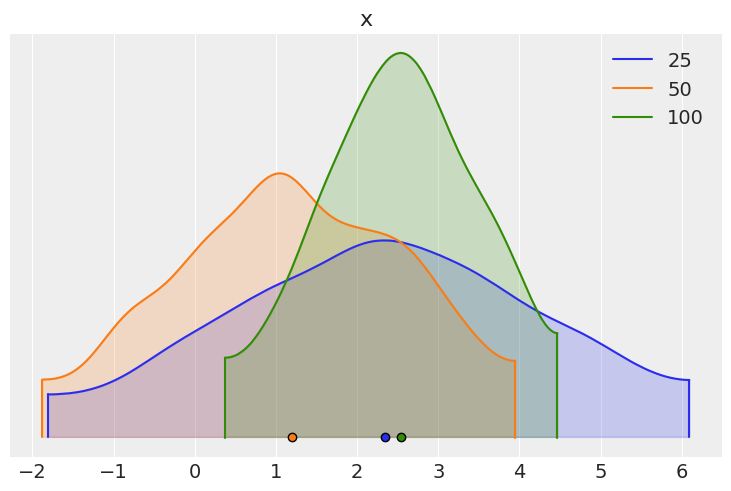
\includegraphics[width=0.8\textwidth]{assets/output.png}
	\caption{Convergencia de los métodos implementados}
\end{figure}
  \item Compare the variance of the estimated slope coefficient obtained form the Monte Carlo simulation with 
    the variance obtained using the asymptotic formula and the variance obtained using a bootstrap method 
    \begin{table}[h]
\centering
\begin{tabular}{c c c c c}
\hline
\textbf{Sample Size} & \textbf{Posterior Var} & \textbf{Asymptotic Var} & \textbf{Bootstrap Var} \\
\hline
25  & 4.587303 & 4.070104 & 3.484380 \\
50  & 2.539172 & 2.327265 & 2.142014 \\
100 & 1.193076 & 1.073991 & 1.129780 \\
\hline
\end{tabular}
\caption{Comparison of variances for different sample sizes}
\label{tab:variance_comparison}
\end{table}

\end{enumerate}
  \begin{pythonbox}[Python Code]
	\inputminted{python}{code/reg5.py}
\end{pythonbox}
\end{document}
